推荐系统是一种常见的信息过滤技术,其评估通常采用公开数据集进行实验,并比较不同模型的实验性能。本章首先将介绍标签感知推荐系统中常用的数据集,以及用于评估的指标。在给出基线模型的对比之后,本章对 LFGCF 和 TAGCL 模型的实验结果分别进行分析。此外,在真实的推荐系统数据上评估了 TAGCL 模型的性能。
%最后,本章将展示一个真实的标签感知推荐系统。

\section{数据集}
本节简要介绍了研究所使用到的数据集。除去三个常用的评估数据意外,本文还在一个真实运行的标签系统数据上评估实验,以佐证模型的有效性。

本文基于三个公开的数据集 MovieLens、Last.FM 和 Delicious 进行实验。这些数据集都在 HetRec2011\cite{cantador_hetrec_2011} 中发布。为了充分验证本文提出的模型 LFGCF 和 TAGCL 在标签感知推荐系统中的表现,本文在一个真实应用的社会化书签和出版物系统 BibSonomy 中进一步验证大规模场景下的模型性能。

(1) \textbf{MovieLens} 是一个电影推荐数据集,来源于电影推荐系统 MovieLens\footnote{https://movielens.org/}。平台上的用户可以为为电影进行打分并且使用任意标签标注电影。MovieLens 数据集中,每一个用户都有一个喜欢的电影的标注列表,本文将电影作为用户的个性化推荐物品。数据集由用户ID,电影ID 和标签ID 组成;

(2) \textbf{Last.fm} 是一个音乐人推荐数据集,来源于著名的电台网站 Last.fm\footnote{https://www.last.fm/}。平台上的用户可以搜索、收藏、评论自己喜欢的音乐,并且可以随意为自己喜欢的音乐标注上个性化的标签。MovieLens 数据集中,每一个用户都有一个喜欢的歌手的标注列表,本文将歌手作为用户的个性化推荐物品。数据集由用户ID,歌手ID 和标签ID 组成;

(3) \textbf{Delicious} 是一个网页书签推荐数据集,来源于提供网络书签管理服务的社交平台 Del.icio.us\footnote{https://del.icio.us/}。平台上的用户可以和其他用户分享、交流网络书签,也可以保持整理自己的私人书签,并鼓励用户为书签进行标注。数据集由用户ID,书签 ID 和标签 ID 组成;

(4) \textbf{BibSonomy} 是一个真实标签系统 BibSonomy\footnote{https://www.bibsonomy.org/} 的数据集,以 SQL 的形式提供给研究人员。平台为用户提供了便捷出版物和网页书签管理方式,并通过社交网络协助寻找潜在的研究方向。数据集可以分为 BibSonomy-BM 与 BibSonomy-BT 两个部分。BibSonomy-BM 由用户 ID,书签 ID 和标签 ID 组成。BibSonomy-BT 由用户 ID,出版物 ID 和标签 ID 组成。

为了降低用户随意标注为数据引入的噪声,本文保持了\cite{zuo_tag-aware_2016}相同的设置,对于 Last.Fm 数据集, 过滤频次少于 5 次的标签;对于 Delicious 数据集,过滤频次少于 15 次的标签;对于 BibSonomy,过滤频次少于 15 次的标签。经过过滤后的数据如表~\ref{data_sta} :

\begin{table}[h]
    \begin{center}
    \caption{数据集统计}
      \begin{tabular}{cccccc}
      \hline
      \textbf{数据集} & \textbf{用户} & \textbf{物品} & \textbf{标签} & \textbf{标注记录} & \textbf{稀疏率} (\%) \\
      \hline
      Last.FM & 1808 & 12212 & 2305 & 175641 & 99.20\% \\
      MovieLens & 1651 & 5381 & 1586 & 36728 & 99.59\% \\
      Delicious & 1843 & 65877 & 3508 & 330744 & 99.73\% \\
      BibSonomy-BM & 5996 & 576232 & 8092 & 1622320 & 99.95\% \\
      BibSonomy-BT & 9721 & 750514 & 9721 & 1972556 & 99.97\% \\
      \hline
      \end{tabular}
    \label{data_sta}
  \end{center}
  \end{table}

由表~\ref{data_sta}~可以看出,Last.FM、MovieLens 与 Delicious 这类的研究型公开数据集,数据规模较小,而真实的运行的标签系统数据规模更大,并且更为稀疏。

% \subsection{数据可视化}

% 1. 统计特征
% 2. 数据bias

\section{实验方法}
本节将介绍本文进行推荐算法实验的实验方法,首先介绍整体实验设计思路,给出实验评估时使用的评估指标,最后简要介绍需要对比的基线模型。
\subsection{实验设计}
推荐系统的设计和实现涉及到多个领域,如机器学习、信息检索、数据挖掘和人工智能等。在推荐系统研究中,实验是不可或缺的一步,实验结果的准确性和可重复性对研究的质量至关重要。本文的实验在一台服务器上进行,硬件配置如下:2颗8核E5-2620V4 2.0GHz,DDR4 ECC REG内存128G,2400MHz;系统硬盘:1块256G SATA SSD;数据硬盘:4TB 企业级硬盘;2块GPU卡(NVIDIA TITAN Xp Pascal)。根据 Dacrema 等人\cite{dacrema_arewe_2019}的调研,同一个模型算法在不同平台上实现可能会导致结果不同,从而增加了实验重复性的难度。因此,本文选择使用一个基于PyTorch实现的推荐系统实验平台RecBole\cite{zhao_recbole_2021},版本为1.0.1。RecBole是一个面向研究者的、易于开发和复现的推荐系统实验平台,提供了统一、全面、高效的推荐系统实验环境。使用RecBole进行实验,可以保证实验结果的可重复性和准确性。最终实验设计流程如下:

(1)数据集选择:在本文实验中,本文选取了 HetRec2011 发布的三个数据集作为实验数据,同时在一个真实运行的推荐系统数据上进行实验;

(2)数据预处理:为了减少冷启动问题和数据噪声对模型训练的影响,我们对数据进行了预处理,其中包括 ID 重映射和低频标注记录过滤等操作;

(3)数据划分:本文将处理后的数据随机划分为训练集、验证集和测试集,其中训练集、验证集和测试集的比例分别为 6:2:2;

(4)模型训练:本文采用 RecBole 实验框架下的基线模型、LFGCF 和 TGCN 进行模型训练,直至损失函数收敛;

(5)模型验证与测试:在验证集上选取效果最优的模型,并在测试集中得到最终推荐结果;

(6)超参数实验:本文对模型进行超参数实验,遍历探索模型最优超参数,并分析超参数灵敏度;

(7)实验分析与总结。最后,本文对实验结果进行了分析与总结,得出了一些有价值的结论和启示。

\subsubsection{评估指标}
为了充分验证和对比模型性能,本文选取了四个在个性化排序推荐领域常见的评估指标:召回率(Recall@K)、准确率(Precision@K)\cite{roelleke_information_2022}、归一化累计折损增益(Normalized Discounted Cumulative Gain,NDCG@K)\cite{wang_theoretical_2013},平均逆排名(Mean Reciprocal Rank,MRR@K)\cite{craswell_mean_2009},以及一个用于评估推荐系统流行度的指标——平均推荐流行度(Average Recommendation Popularity,ARP@K)\cite{yin_challenging_2012}。这些指标与标签感知推荐系统的性能和最终的Top-K推荐列表的质量密切相关,其中除去平均推荐流行度以外的指标数值越高,则表示模型性能越优秀。

召回率和准确率的计算方法源自于评估分类状况的混淆矩阵(Confusion Matrix)。混淆矩阵是机器学习中用于评估分类器性能的一种工具。它是一个二维的表格,横轴代表预测值,纵轴代表实际值。每个单元格代表预测结果为横轴类别,实际结果为纵轴类别的样本数。混淆矩阵通过计数真正的阳性(True Positive,TP)、假阴性(False Negative,FN)、假阳性(False Positive,FP)和真正的阴性(True Negative,TN)来评估分类器的准确性。这些信息可以计算出多种分类指标,例如准确率(Accuracy)、召回率(Sensitivity)、等。表\ref{tab:confusion_matrix}为一个二分类的混淆矩阵。

\begin{table}[htbp]
  \centering
  \caption{二分类混淆矩阵}
  \label{tab:confusion_matrix}
  \begin{tabular}{ccc}
  \hline
  \multirow{2}{*}{实际值} & \multicolumn{2}{c}{预测值} \\ \cline{2-3}
  & 正类 & 负类 \\ \hline
  正类 & TP & FN \\
  负类 & FP & TN \\ \hline
  \end{tabular}
\end{table}
基于混淆矩阵,召回率和准确率可以被定义为:
\begin{equation}
  \begin{aligned}
    R &= \frac{TP}{TP + FN}, \\
    P &= \frac{TP}{TP + FP}
  \end{aligned}
\end{equation}
在此基础上,个性化推荐系统的召回率和准确率根据具体应用场景有着进一步改进。其中召回率衡量的是系统推荐给用户的物品中,用户实际发生交互的物品数量与系统推荐给用户的物品的比值。该指标为推荐系统最为重要的指标,本文在验证集上选取召回率最高的模型作为测试模型。召回率可以被定义为:
\begin{equation}
  Recall@K = \frac{|R^N(u) \bigcap T(u)|}{|T(u)|}
\end{equation}
其中,$T(u)$ 表示系统推荐给用户的物品的数量,$R^N(u)$ 用户实际发生交互的物品数量,$Recall@N$ 中的 $K$ 指个性化推荐列表的长度。

准确率则描述的是是系统推荐给用户的物品中,用户实际发生交互的物品数量与用户实际发生交互物品的比值。准确率可以被定义为:
\begin{equation}
  Precision@K = \frac{|R^N(u) \bigcap T(u)|}{N}
\end{equation}
其中,$N$ 表示用户在系统中实际交互过的物品数量,$R^N(u)$ 用户实际发生交互的物品数量,$Precision@N$ 中的 $K$ 指个性化推荐列表的长度。

归一化累计折损增益是一种评估排名效果的指标,常用于搜索引擎、推荐系统等领域。它通过计算排名中每个项目的得分权重,以评估排名的质量。NDCG 的优点在于它可以评估排名的相对质量,并且可以适用于任意数量的排名项目。它是一种规范化的指标,因此可以在不同的应用场景中进行比较。
\begin{equation}
  nDCG@K = \frac{1}{\mathcal{U}}\sum_{u \in \mathcal{U}} \frac{\sum^N_{n=1} \frac{I(R^N_n(u) \in T(u))}{log(n+1)}}{\sum^N_{n=1}\frac{1}{log(n+1)}}
\end{equation}
其中 $R^N_n(u)$ 指 Top-K 推荐中的第 $n^{th}$ 项用户发生交互的物品 $R^N(u)$,$NDCG@N$ 中的 $K$ 指个性化推荐列表的长度。

平均逆排名是一种常用于信息检索与推荐系统负评估指标,用于评估查询结果的质量。它通过计算正确检索结果在检索列表中的排名来评估系统性能。
\begin{equation}
  MRR@K = \frac{1}{\mathcal{U}} \sum_{u \in \mathcal{U}}\frac{1}{rank_u^*}
\end{equation}
其中,$rank_u^*$表示对用户的推荐中第一个相关项目的排名位置。

为评估推荐系统中存在的流行度偏差带来的不公平现象,本文额外使用平均推荐流行度是否降低了对热门物品的推荐偏见。其通过计算模型推荐给用户的物品,其在训练数据中流行度的平均值,以评估模型是否对于热门物品更为偏好。
\begin{equation}
  AveragePopularity@K=\frac{1}{|U|} \sum_{u \in U } \frac{\sum_{i \in R_{u}} \phi(i)}{|R_{u}|}
\end{equation}
其中 $\phi(i)$ 指物品 $i$ 在训练数据的被交互次数。与本文其他用到的指标不同,平均推荐流行度越低,代表模型的推荐能力越优秀。

\subsection{对比模型}
为了综合对比评估推荐模型的性能,本文比较了通用的推荐算法模型和标签感知推荐算法模型。其中,通用推荐算法模型采用了基于图神经网络的推荐算法中常用的基准模型LightGCN\cite{he_lightgcn_2020}和基于图对比学习的SimGCL\cite{yu_simgcl_2022};标签感知的推荐算法模型则采用了BPR-T\cite{li_tag-aware_2019}和基于图神经网络算法的TGCN\cite{chen_tgcn_2020}。模型具体介绍如下:

(1)\textbf{LightGCN} 是一种广泛使用的基准模型,因其简单性和有效性而受到推荐系统领域的青睐。它采用了一种去除非线性激活函数的简单图神经网络进行表征学习,从而对推荐系统中的用户和物品进行建模;

(2)\textbf{SimGCL} 与常见的对图数据进行增强以进行对比学习任务的方法不同,它对嵌入表征进行扰动,以构建对比学习任务。该模型的主干网络采用了LightGCN的设计,进一步提升了模型的性能;

(3)\textbf{BPR-T} 通过改进BPR损失函数,将用户标注行为引入协同过滤模型中,提高了推荐系统的性能。具体而言,BPR-T将标签信息作为用户行为的一部分来进行建模,从而更准确地预测用户对物品的偏好;

(4)\textbf{TGCN} 构建了一个复杂的图卷积模型,利用注意力机制和卷积神经网络增强了模型的特征学习能力,使得标签感知推荐系统第一次运用了图神经网络。该模型能够准确地捕捉用户和物品之间的关系,从而更好地进行推荐。

\section{实验评估}
本节将介绍基线模型、LFGCF和TAGCL在MovieLens、Last.FM和Delicious数据集上的实验结果,并对LFGCF和TAGCL进行详细的消融实验,以进一步比较模型设计的优劣。
\subsection{实验设置}
为了保证实验的公平性,本文使用基于Minibatch设置下的Adam优化器\cite{kingma_adam_2014}来训练所有模型,BatchSize设置为2048,并将模型的最大训练轮数设置为500轮,同时采用早停机制\cite{prechelt_early_2012}来避免过拟合的问题。本文使用网格法搜索最佳超参数,其中学习率的搜索范围为\{0.0005、0.001、0.005、0.01\},正则化权重的搜索范围为\{1e-5、1e-4、1e-3、1e-2\}。对于所有需要嵌入表征的模型,嵌入表征维度设置为 64,并通过最常用的Xavier方式\cite{glorot_understanding_nodate}进行随机初始化。推荐序列长度均设置为 20。其余基线模型的性能按照原始论文的报告进行调整。

\subsection{性能对比实验分析}
最终模型的个性化推荐性能如表~\ref{tab:movielens_performance_comparison}、\ref{tab:lastfm_performance_comparison}、\ref{tab:delicious_performance_comparison}~所示。其中,imp. 指提高的百分比,黑体高亮的数字指所有模型中最好的性能,下划线指标签感知推荐系统中最高的性能。结果表明,LFGCF 和 TAGCL 在大部分指标中都优于基线模型。在标签感知推荐的模型中,LFGCF 依靠轻量化设计的图神经网络结构,比起直接使用原始图神经网络的 TGCN,有着更强的性能。由于模型在更短的训练轮次内就收敛了,所以可以获得更稳健的嵌入表征,从而得到更稳定的表现。同时,LFGCF 也依靠图神经网络的设计,在消息传播过程中获取了丰富的上下文信息,缓解了标签感知推荐系统这一特有问题中的一次多义和多次同义的问题。而 TAGCL 则进一步优化了当数据存在大量偏差时模型的性能,尤其是在 Last.FM 和 MovieLens 这两个数据集中存在大量偏见时。但是在数据集 Delicious 中存在较少偏差时,TAGCL 的性能稍有损失。

对于基线模型而言,通用推荐模型 SimGCL 在大多数指标中都优于 LightGCN。这是因为 SimGCL 使用对比学习改进了 LightGCN 在训练时,损失函数偏向于拟合数据集的结果而不是寻找用户和物品之间的交互规律。而在标签感知推荐算法中,虽然 TGCN 使用了图神经网络这一更新深度学习技术,但并没有针对标签推荐做出优化。因此,在部分指标中,TGCN 和 BPR-T 相比并没有显著的优势。
\subsubsection{MovieLens 结果分析}
表~\ref{tab:movielens_performance_comparison} 为数据集 MovieLens 下的模型对比实验。本表中列出了在 MovieLens 数据集上的六种不同的推荐模型,包括通用推荐模型(LightGCN和SimGCL),标签感知推荐模型(BPR-T和TGCN),LFGCF 和 TAGCL。从评估指标来看,TAGCL 在五个指标中均取得了最佳的结果。其中,TAGCL 在 Pre. 上的表现最好,达到了 0.0405;在 NDCG 上,TAGCL 取得了 0.2338 的分数,排名第一;在 MRR 上,TAGCL 的得分为 0.2356,排名第二;在 Rec. 和 ARP 指标上,TAGCL 分别排名第二和第一。此外,LFGCF 在 Rec. 和 ARP 指标上的表现相对较差,分别排名第四和第五,但在 Prec. 上表现不错,排名第二。SimGCL 在 Prec. 上的表现相对较差,排名第四,但在 NDCG 和 MRR 上的表现较好,排名第二和第三。BPR-T 在五个指标中排名第三,相对而言表现较为平衡。LightGCN 和 TGCN 在五个指标中排名较中等,表现不如其他模型。
\begin{table}[!h]
  \caption{数据集 MovieLens 下的模型对比实验}
  \centering
  \label{tab:movielens_performance_comparison}
  \begin{tabular}{c|c|c|c|c|c|c|c|c}
      \toprule
      \multirow{2}{*}{\textbf{指标}} & 
      \multicolumn{2}{c|}{\textbf{通用推荐}} & 
      \multicolumn{2}{c|}{\textbf{标签感知推荐}} & 
      \multirow{2}{*}{\textbf{LFGCF}} & 
      \multirow{2}{*}{\textbf{TAGCL}} & 
      \multirow{2}{*}{\textbf{imp. SOTA}} & 
      \multirow{2}{*}{\textbf{imp. TRS}} \\
      \cline{2-5}
      & \textbf{LightGCN} & \textbf{SimGCL} 
      & \textbf{BPR-T} & \textbf{TGCN}  & & & & \\
      \midrule
      \begin{tabular}[c]{@{}c@{}}
          Rec. \\ Pre. \\ NDCG \\ MRR \\ ARP
        \end{tabular} & 
        \begin{tabular}[c]{@{}c@{}} % LightGCN
          0.2788 \\ 0.0349 \\ 0.2015 \\ 0.2101 \\ 26.78
        \end{tabular} & 
        \begin{tabular}[c]{@{}c@{}} % simgcl
          0.2835 \\ \underline{0.0383} \\ \underline{0.2274} \\ \textbf{0.2383} \\ 18.15
        \end{tabular} &
        \begin{tabular}[c]{@{}c@{}} % bprt
          0.2826 \\ 0.0365 \\ 0.2209 \\ 0.2273 \\ 22.76
        \end{tabular} &
        \begin{tabular}[c]{@{}c@{}} % tgcn
          0.2812 \\ 0.0372 \\ 0.2187 \\ 0.2218 \\ 25.25
        \end{tabular} &
        \begin{tabular}[c]{@{}c@{}} % lfgcf
          \underline{0.2929} \\ 0.0365 \\ 0.2140 \\ 0.2183 \\ \underline{18.10}
        \end{tabular} &
        \begin{tabular}[c]{@{}c@{}} % tagcl
          \textbf{0.3180} \\ \textbf{0.0405} \\ \textbf{0.2338} \\ \underline{0.2356} \\ \textbf{14.96}
        \end{tabular} &
        \begin{tabular}[c]{@{}c@{}}
          8.57\% \\ 5.74\% \\ 2.81\% \\ -1.13\% \\ 17.07\%
        \end{tabular} &
        \begin{tabular}[c]{@{}c@{}}
          8.57\% \\ 8.87\% \\ 5.84\% \\ 3.65\% \\ 17.58\%
        \end{tabular} \\
        \bottomrule
  \end{tabular}
\end{table}


\subsubsection{Last.FM 结果分析}
表~\ref{tab:lastfm_performance_comparison} 为数据集 Last.FM 下的模型对比实验。从表格可以看出,TAGCL 在五项指标中表现最好,Rec.、Pre.、NDCG、MRR 和 ARP 分别为 0.5199、0.1611、0.4949、0.5541 和 42.99。其次是 SimGCL,在 Pre.、NDCG、MRR 和 ARP 方面略逊于 TAGCL,但推荐精度最高,达到了 0.5055。LFGCF 在推荐精度和 NDCG 方面略高于 SimGCL,但在其他指标方面稍逊于 SimGCL。BPR-T 和 TGCN 在所有指标中表现最差,其中 BPR-T 在推荐精度和 NDCG 方面略好于 TGCN,但在其他指标方面略逊于 TGCN。
\begin{table}[!h]
  \caption{数据集 Last.FM 下的模型对比实验}
  \centering
  \label{tab:lastfm_performance_comparison}
  \begin{tabular}{c|c|c|c|c|c|c|c|c}
      \toprule
      \multirow{2}{*}{\textbf{指标}} & 
      \multicolumn{2}{c|}{\textbf{通用推荐}} & 
      \multicolumn{2}{c|}{\textbf{标签感知推荐}} & 
      \multirow{2}{*}{\textbf{LFGCF}} & 
      \multirow{2}{*}{\textbf{TAGCL}} & 
      \multirow{2}{*}{\textbf{imp. SOTA}} & 
      \multirow{2}{*}{\textbf{imp. TRS}} \\
      \cline{2-5}
      & \textbf{LightGCN} & \textbf{SimGCL} 
      & \textbf{BPR-T} & \textbf{TGCN}  & & & & \\
      \midrule
      \begin{tabular}[c]{@{}c@{}}
          Rec. \\ Pre. \\ NDCG \\ MRR \\ ARP
        \end{tabular} & 
        \begin{tabular}[c]{@{}c@{}} % LightGCN
          0.4835 \\ 0.1375 \\ 0.4087 \\ 0.4664 \\ 111.99
        \end{tabular} & 
        \begin{tabular}[c]{@{}c@{}} % simgcl
          0.5055 \\ \underline{0.1534} \\ \underline{0.4680} \\ \underline{0.5263} \\ \underline{51.67}
        \end{tabular} &
        \begin{tabular}[c]{@{}c@{}} % bprt
          0.4714 \\ 0.1363 \\ 0.4321 \\ 0.5083 \\ 103.74
        \end{tabular} &
        \begin{tabular}[c]{@{}c@{}} % tgcn
          0.4736 \\ 0.1332 \\ 0.4225 \\ 0.4874 \\ 78.88
        \end{tabular} &
        \begin{tabular}[c]{@{}c@{}} % lfgcf
          \underline{0.5057} \\ 0.1465 \\ 0.4482 \\ 0.5033 \\ 80.65
        \end{tabular} &
        \begin{tabular}[c]{@{}c@{}} % tagcl
          \textbf{0.5199} \\ \textbf{0.1611} \\ \textbf{0.4949} \\ \textbf{0.5541} \\ \textbf{42.99}
        \end{tabular} &
        \begin{tabular}[c]{@{}c@{}}
          2.81\% \\ 5.02\% \\ 5.75\% \\ 5.28\% \\ 16.80\%
        \end{tabular} &
        \begin{tabular}[c]{@{}c@{}}
          2.81\% \\ 9.97\% \\ 10.42\% \\ 9.01\% \\ 46.70\%
        \end{tabular} \\
        \bottomrule
  \end{tabular}
\end{table}

\subsubsection{Delicious 结果分析} 
表~\ref{tab:delicious_performance_comparison} 为数据集 Delicious 下的模型对比实验。从表格中可以看出,对于通用推荐任务,LightGCN 和 SimGCL 的表现非常接近,但在 NDCG 和 MRR 两个指标上,LightGCN 略胜一筹。对于标签感知推荐任务,BPR-T 和 TGCN 的表现也很接近,但在 Rec. 和 Pre. 两个指标上,TGCN 的表现略优于 BPR-T。同时,LFGCF 和 TAGCL 这两种改进模型相比通用推荐和标签感知推荐的基准模型都有明显的提升,其中 TAGCL 在所有指标上都取得了最佳的结果。综上所述,本实验中 LFGCF 和 TAGCL 这两种改进模型在 Delicious 数据集上表现最优,可以作为该数据集上推荐系统的首选模型。
\begin{table}[!h]
  \caption{数据集 Delicious 下的模型对比实验}
  \centering
  \label{tab:delicious_performance_comparison}
  \begin{tabular}{c|c|c|c|c|c|c|c|c}
      \toprule
      \multirow{2}{*}{\textbf{指标}} & 
      \multicolumn{2}{c|}{\textbf{通用推荐}} & 
      \multicolumn{2}{c|}{\textbf{标签感知推荐}} & 
      \multirow{2}{*}{\textbf{LFGCF}} & 
      \multirow{2}{*}{\textbf{TAGCL}} & 
      \multirow{2}{*}{\textbf{imp. SOTA}} & 
      \multirow{2}{*}{\textbf{imp. TRS}} \\
      \cline{2-5}
      & \textbf{LightGCN} & \textbf{SimGCL} 
      & \textbf{BPR-T} & \textbf{TGCN}  & & & & \\
      \midrule
      \begin{tabular}[c]{@{}c@{}}
          Rec. \\ Pre. \\ NDCG \\ MRR \\ ARP
        \end{tabular} & 
        \begin{tabular}[c]{@{}c@{}} % LightGCN
          0.3337 \\ 0.3525 \\ \underline{0.4213} \\ \underline{0.5786} \\ \textbf{3.11}
        \end{tabular} & 
        \begin{tabular}[c]{@{}c@{}} % simgcl
          \underline{0.3351} \\ \underline{0.3554} \\ 0.4177 \\ 0.5529 \\ \underline{4.67}
        \end{tabular} &
        \begin{tabular}[c]{@{}c@{}} % bprt
          0.3150 \\ 0.3409 \\ 0.3984 \\ 0.5373 \\ 6.32
        \end{tabular} &
        \begin{tabular}[c]{@{}c@{}} % tgcn
          0.3284 \\ 0.3519 \\ 0.4160 \\ 0.5589 \\ 6.21
        \end{tabular} &
        \begin{tabular}[c]{@{}c@{}} % lfgcf
          0.3300 \\ 0.3498 \\ 0.4080 \\ 0.5395 \\ 4.69
        \end{tabular} &
        \begin{tabular}[c]{@{}c@{}} % tagcl
          \textbf{0.3432} \\ \textbf{0.3705} \\ \textbf{0.4385} \\ \textbf{0.5828} \\ 5.61
        \end{tabular} &
        \begin{tabular}[c]{@{}c@{}}
          2.42\% \\ 4.25\% \\ 4.08\% \\ 0.73\% \\ -80.39\%
        \end{tabular} &
        \begin{tabular}[c]{@{}c@{}}
          4.00\% \\ 5.29\% \\ 5.41\% \\ 4.28\% \\ -19.62\%
        \end{tabular} \\
      \bottomrule
  \end{tabular}
\end{table}

\subsection{LFGCF 模型评估}
本节在 Last.FM 与 Delicious 数据集上,对 LFGCF 进行消融实验以进一步理解各个组件是如何影响其性能的。表~\ref{tab:lfgcf_ablation}~展示了 LFGCF 与其变体的性能比较。其中,LFGCF-L 指未使用轻量化图神经网络的变体,LFGCF-T 指未使用知识图谱的 TransRT 正则化的变体。

\begin{table}	[!h]
	\centering
	\begin{subtable}[t]{0.49\linewidth}
		\centering
        \begin{tabular}{ccc}
            \toprule
            \textbf{模型} & \textbf{Recall@10} &  \textbf{Recall@20} \\
            \midrule
            \begin{tabular}[c]{@{}c@{}}
                LFGCF-L \\ LFGCF-T \\ LFGCF
            \end{tabular} 
            & \begin{tabular}[c]{@{}l@{}}
                0.4208 \\0.4336 \\ 0.4362 
            \end{tabular}
            & \begin{tabular}[c]{@{}l@{}}
                0.4958 \\0.5027 \\ 0.5132
            \end{tabular} \\
            \bottomrule
        \end{tabular} 
        \caption{数据集 Last.FM 下的 LFGCF 消融实验} \label{tab:lastfm_lfgcf_ablation}
	\end{subtable}
  \begin{subtable}[t]{0.49\linewidth}
		\centering
  \begin{tabular}{ccc}
            \toprule
            \textbf{模型} & \textbf{Recall@10} &  \textbf{Recall@20} \\
            \midrule
            \begin{tabular}[c]{@{}c@{}}
                LFGCF-L \\ LFGCF-T \\ LFGCF
            \end{tabular} 
            & \begin{tabular}[c]{@{}l@{}}
                0.1615 \\ 0.1903 \\ 0.1955
            \end{tabular}
            & \begin{tabular}[c]{@{}l@{}}
                0.2838 \\ 0.3270 \\ 0.3286
            \end{tabular} \\
            \bottomrule
        \end{tabular} 
\caption{数据集 Delicious 下的 LFGCF 消融实验} \label{tab:delicious_lfgcf_ablation}
\end{subtable}
\caption{LFGCF 消融实验}\label{tab:lfgcf_ablation}
\end{table}

\subsubsection{轻量化图神经网络设计的影响}
在 LFGCF 模型中,本文使用了轻量化的图神经网络以获取大众标注图中的潜在特征。相较于普通的图神经网络,我们去除了非线性激活函数以及特征变换。这样的设计为 LFGCF 带来了显著的性能提升。为了验证该设计的有效性,我们使用了以 NGCF 为主干网络的模型 LFGCF-L 作为比较。表~\ref{tab:lastfm_lfgcf_ablation}~可见,在数据集 Last.FM 下,LFGCF-L 是未使用轻量化图神经网络的变体,它的 Recall@10 和 Recall@20 分别为 0.4208 和 0.4958,相对较低。表~\ref{tab:delicious_lfgcf_ablation}~可见,在数据集 Delicious 下,LFGCF 在数据集 Delicious 中的性能更加显著,其 Recall@10 和 Recall@20 分别为 0.1615 和 0.2838。这表明在 Delicious 数据集上,轻量化图神经网络的设计对于学习用户和物品自身的嵌入表征是非常有效的。这意味着 LFGCF 的轻量化设计可以有效地获取大众标注图中的潜在特征。
\subsubsection{TransRT 设计的影响}
在 LFGCF 模型中,本文使用了基于知识图谱的 TransRT,在优化时发挥作用。其通过标签,将用户和物品统一到同一向量空间的设计为 LFGCF 解决了标签感知推荐系统中的一次多义、多词同义问题。我们将去除了 TransRT 这一组件的 LFGCF 记为 LFGCF-T。表~\ref{tab:lastfm_lfgcf_ablation}~可见,在数据集 Last.FM 下,LFGCF 取得了最好的 Recall@10 和 Recall@20 分数,分别为 0.4362 和 0.5132。表~\ref{tab:delicious_lfgcf_ablation}~可见,在数据集 Delicious 下,LFGCF 的性能略高于 LFGCF-T,说明 TransRT 正则化对于解决标签感知推荐系统中的多义、多词同义问题是非常有效的。总体而言,在两个数据集上,LFGCF 的性能最好,LFGCF-T 的性能略低于 LFGCF。这表明使用基于知识图谱的 TransRT 正则化可以提高 LFGCF 的性能。虽然 LFGCF 的性能略高于 LFGCF-T,但二者之间的性能差异很小,表明 LFGCF 的轻量化图神经网络设计已经非常有效。

\subsection{TAGCL 模型评估}
本节在 Last.FM 与 Delicious 数据集上,对 TAGCL 进行消融实验以进一步理解各个组件是如何影响其性能的。表~\ref{tab:tagcl_ablation}~展示了 TAGCL 与其变体的性能比较。其中,TAGCL-A 等价于 LFGCF-T,是一个仅包含基本图结构的基线模型,TAGCL-CL 去掉了框架中的对比学习任务,TAGCL-NT 去掉了框架中的标签副采样过程,TAGCL-T 则去掉了基于知识图谱的 TransT 正则化。
\begin{table}[!h]
	\centering
	\begin{subtable}[t]{0.49\linewidth}
		\centering
        \begin{tabular}{ccc}
            \toprule
            \textbf{模型} & \textbf{Rec.@20} & \textbf{ARP.@20} \\
            \midrule
            \begin{tabular}[c]{@{}c@{}}
                TAGCL-A \\ TAGCL-CL \\ TAGCL-NT \\ TAGCL-T \\ TAGCL
              \end{tabular} &
              \begin{tabular}[c]{@{}c@{}} % recall
                0.4502 \\ 0.4141 \\ \textbf{0.5212} \\ 0.5193 \\ 0.5199
              \end{tabular} &
              \begin{tabular}[c]{@{}c@{}} % ARP
                92.05 \\ 89.42 \\ 43.92 \\ 52.17 \\ \textbf{42.99}
              \end{tabular} \\
            \bottomrule
        \end{tabular} 
        \caption{数据集 Last.FM 下的 TAGCL 消融实验} \label{tab:lastfm_tagcl_ablation}
	\end{subtable}
  \begin{subtable}[t]{0.49\linewidth}
		\centering
		% \label{tab:delicious_lfgcf_ablation}
    \begin{tabular}{ccc}
        \toprule
        \textbf{模型} & \textbf{Rec.@20} & \textbf{ARP.@20} \\
        \midrule
        \begin{tabular}[c]{@{}c@{}}
            TAGCL-A \\ TAGCL-CL \\ TAGCL-NT \\ TAGCL-T \\ TAGCL
          \end{tabular} &
          \begin{tabular}[c]{@{}c@{}} % recall
            0.3188 \\ 0.3301 \\ 0.3425 \\ 0.3396 \\ \textbf{0.3432}
          \end{tabular} &
          \begin{tabular}[c]{@{}c@{}} % ndcg
            5.33 \\ \textbf{5.24} \\ 5.48 \\ 5.58 \\ 5.61
          \end{tabular} \\
        \bottomrule
    \end{tabular} 
		\caption{数据集 Delicious 下的 TAGCL 消融实验} \label{tab:delicious_tagcl_ablation}
	\end{subtable}
	\caption{TAGCL 消融实验}\label{tab:tagcl_ablation}
\end{table}

在 Last.FM 数据集上的实验结果在表~\ref{tab:lastfm_tagcl_ablation}~展示,TAGCL-NT 取得了最好的 Rec.@20 得分(0.5212),但是在 ARP.@20 得分方面,TAGCL 取得了最好的成绩(42.99)。这意味着 TAGCL 在前 20 个推荐结果中的平均排名位置最佳。TAGCL-CL 在两个指标上都表现不如 TAGCL 和 TAGCL-NT,这表明对比学习任务对模型性能的贡献很大。

在 Delicious 数据集上的实验结果在表表~\ref{tab:delicious_tagcl_ablation}~展示,TAGCL 取得了最好的 Rec.@20 得分(0.3432),但是在 ARP.@20 得分方面,TAGCL-CL 取得了最好的成绩(5.24)。这表明在不同的数据集上,TAGCL 模型的变体会有不同的表现,但总体而言,TAGCL 在 Rec.@20 和 ARP.@20 上都取得了最佳的成绩,表明该模型在推荐任务中表现优异。

\subsubsection{对比学习的影响}
在 TAGCL 框架中,本文采用一种简单的方式实现对比学习。与常见的对比学习实现思路不同,本文没有使用复杂的图数据增强,而是通过对训练过程中的嵌入表征进行噪声扰动来构建对比学习任务。在 InfoNCE 损失函数的帮助下,TAGCL 取得了优秀的推荐性能。为了验证本文使用的特征增强方式与 InfoNCE 损失函数的有效性,我们首先移除了 TAGCL 中的对比学习任务,得到了TAGCL-CL。同时保持 TAGCL-CL 的超参数与 TAGCL 相同,我们对 TAGCL 模型与其变体 TAGCL-CL 进行了实验,结果如表~\ref{tab:tagcl_ablation}所示。从数据可以看出,由于对比学习任务的加入,TAGCL 模型的性能会显著提高。相比于 TAGCL-A,一个包含 TAGCL 基本图结构的基线模型,TAGCL 的表现更加优秀。因此,对比学习任务对 TAGCL 模型的性能有着巨大贡献。

\subsubsection{负标签采样的影响}
本文提出了一个新的视角,探讨了标签在标签感知推荐系统中的作用。在训练过程中,通过对标签域和物品域进行负采样,并利用物品-标签对配对损失来帮助模型从偏差较小的标签信息中学习到物品的嵌入表征。对去负标签采样的模型进行消融实验,将其记为 TAGCL-NT。实验结果显示,TAGCL-NT 略低于 TAGCL,但仍能胜过 TAGCL-CL 和 TAGCL-A。这表明负标签损失在 TAGCL 中的作用相对不那么关键。虽然标签负向采样对性能提升的贡献较小,但在数据量较大的 Delicious 数据集上,它可以大大提高模型的收敛效率,训练过程从 85 轮减少到 67 轮。

另外,本文引入了 TransT 正则化损失函数,作为促进推荐系统公平性的另一个组件。基于构建的图结构,TransT 正则化可以在用户和物品之间建立桥梁。通过去除 TransT 正则化损失,建立 TAGCL-T 进行实验。结果表明 TransT 正则化是有效的,并且比负标签损失对 TAGCL 的性能提升贡献更大。因此,TAGCL 通过将二元图之间的标签嵌入差异视为连接用户和项目的关系表示,设法统一不同图上的用户和项目嵌入。

\subsubsection{超参数的影响}
本文对标签感知推荐系统中标签的作用进行了探究,并对 TAGCL 方法的参数进行了灵敏度分析。在 Last.FM 和 Delicious 数据集上,我们分别调整了 GNN 的层数和嵌入表征的维度大小,以评估不同参数对 TAGCL 方法的影响。详细的实验结果展示在图图~\ref{fig:tagcl_param_layer}中。

在图~\ref{fig:tagcl_param_layer}中,我们展示了 TAGCL 方法在不同层数下在 Last.FM 和 Delicious 数据集上的准确率。结果表明,增加 GNN 的层数并不总是能提高 TAGCL 的推荐性能。事实上,当 GNN 层数超过三层时,Last.FM 数据集的准确率急剧下降。在 Delicious 数据集上,虽然 Recall@20 和 ARP@20 随着层数的增加而变化,但并没有出现明显的断崖式下降。另外,在层数为两层时,TAGCL 方法在公平性方面表现出较优越的性能。

\begin{figure}[!h]
  \centering
  \begin{subfigure}{0.49\linewidth}
      \centering
      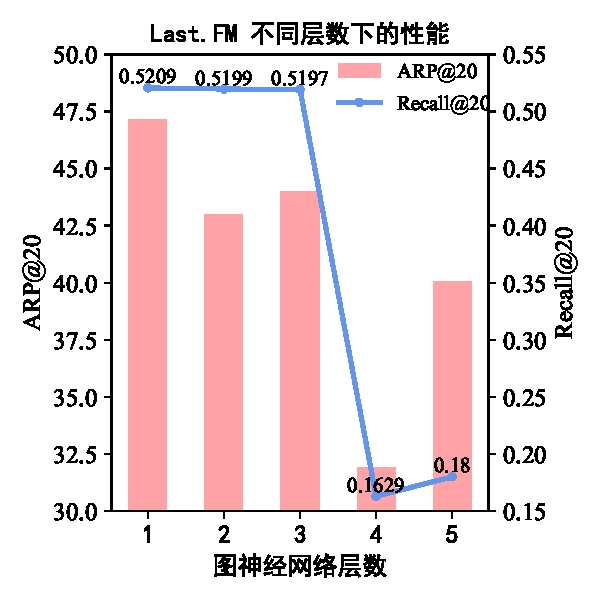
\includegraphics[width=.88\linewidth]{figure/tagcl_param_lastfm_layer.pdf}
      \caption{Last.FM 数据层数对 TAGCL 性能的影响}
      \label{fig:tagcl_param_lastfm_layer}
  \end{subfigure}
  \begin{subfigure}{0.49\linewidth}
    \centering
    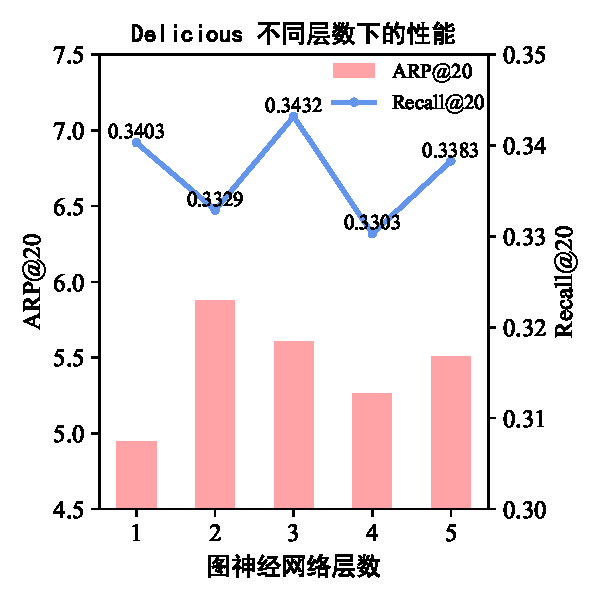
\includegraphics[width=.88\linewidth]{figure/tagcl_param_de_layer.pdf}
    \caption{Delicious 数据层数对 TAGCL 性能的影响}
    \label{fig:tagcl_param_de_layer}
\end{subfigure}
  \caption{图神经网络层数对 TAGCL 性能的影响}
  \label{fig:tagcl_param_layer}
\end{figure}

\begin{figure}[!h]
  \centering
  \begin{subfigure}{0.49\linewidth}
    \centering
    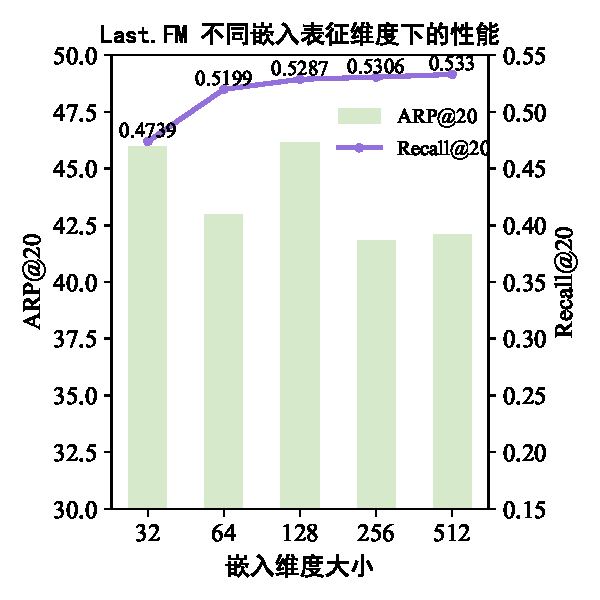
\includegraphics[width=.88\linewidth]{figure/tagcl_param_lastfm_emb.pdf}
    \caption{Last.FM 嵌入表征维度大小对 TAGCL 性能的影响}
    \label{fig:tagcl_param_lastfm_emb}
  \end{subfigure} 
  \begin{subfigure}{0.49\linewidth}
      \centering
      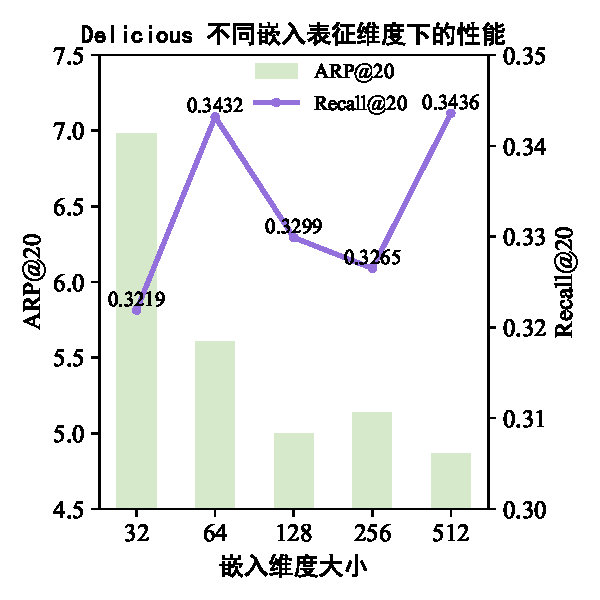
\includegraphics[width=.88\linewidth]{figure/tagcl_param_de_emb.pdf}
      \caption{Delicious 嵌入表征维度大小对 TAGCL 性能的影响}
      \label{fig:tagcl_param_de_emb}
  \end{subfigure}
  \caption{嵌入表征维度大小对 TAGCL 性能的影响}
  \label{fig:tagcl_param_emb}
\end{figure}


此外,我们还研究了嵌入表征的维度大小对 TAGCL 方法的影响。实验结果展示在图~\ref{fig:tagcl_param_emb} 中。在 Last.FM 数据集上(图~\ref{fig:tagcl_param_lastfm_emb}~),我们发现随着嵌入规模的增加,TAGCL 方法的推荐准确率也随之增加。而在 Delicious 数据集上(图~\ref{fig:tagcl_param_de_emb}~),TAGCL 的推荐性能则在嵌入规模变化时表现出较大的波动。特别地,当嵌入规模较大时,TAGCL 方法在 Delicious 数据集上表现更具有公平性。综合考虑性能和效率,我们认为使用 64 的嵌入尺寸是 TAGCL 方法的最佳选择。

\subsubsection{个性化序列长度对模型的影响}
本节旨在探索不同个性化序列长度对 TAGCL 推荐性能的影响。为此,我们分析了数据集 Last.FM 和 Delicious 下,TAGCL 在不同个性化序列长度 $K$ 下与其他基线模型的推荐性能。我们的实验结果显示,TAGCL 在 Recall 和 NDCG 两个指标下,在任意个性化序列长度 $K$ 下均有显著的性能提升,特别是在 NDCG 中,TAGCL 相对于次优模型有约 5\% 的提升。此外,TAGCL 对流行性偏差也有较强的抑制作用,在任意个性化序列长度 $K$ 下均表现出最低的偏差。然而,Delicious 数据集由于数据流行度偏差较小,因此该指标 TAGCL 并没有明显优势。总之,我们的实验结果表明,个性化序列长度 $K$ 对于 TAGCL 推荐性能有着显著的影响,并且该模型能够有效地抑制流行性偏差,提高推荐质量。
\begin{figure}[!h]
  \centering
  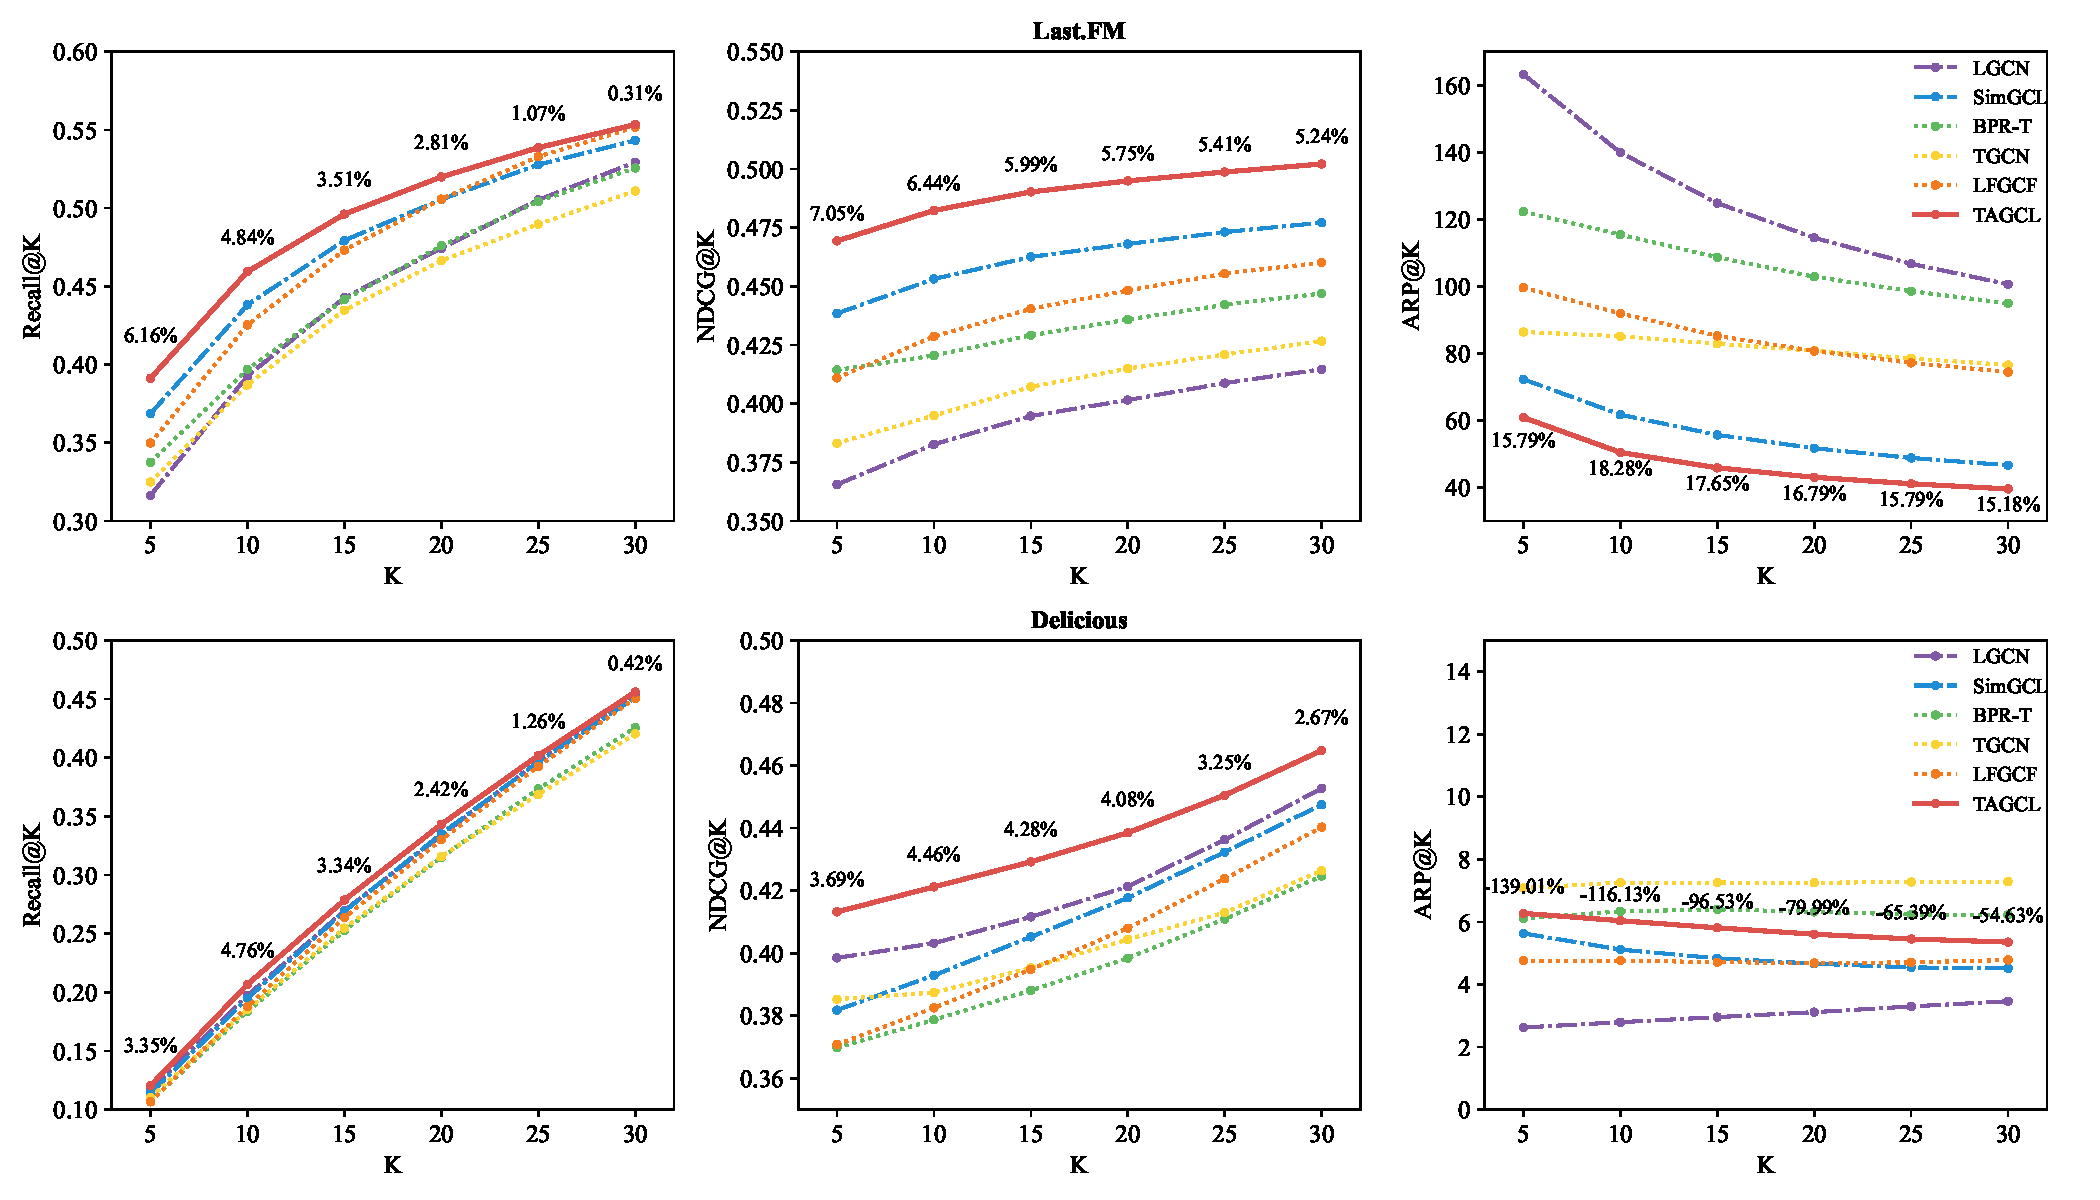
\includegraphics[width=1\linewidth]{figure/topk_comparison.pdf}
  \caption{不同个性化序列长度下的 TAGCL 推荐性能}
  \label{fig:topk}
\end{figure}

\subsection{模型复杂度分析}
本文量化分析了 LFGCF 的参数与推理时间复杂度,并且比较了模型参数量与推理时间。表~\ref{tab:complexity} 展示了 LFGCF 和其他基线模型的参数量与推理时间。与其他标签感知模型相比,LFGCF的参数数量最少,因为它只需要学习用户、项目和标签的嵌入。因此,LFGCF 的参数比一般的模型多。我们的嵌入表征近包含标签嵌入,它提供了大约$0.22 \times 10^6$ 的可训练参数。由于大规模的推荐系列通常对延迟有很高的要求,推理过程中的计算成本很重要。表~\ref{tab:complexity}显示,大多数模型需要大约$0.15s$来推理 Delicious 中的所有测试集。然而,TGCN 明显比其他模型慢,因为它的重特征聚合设计,获得了注意力机制和卷积神经网络。

\begin{table}[!h]
  \centering
    \caption{模型在 Delicious 上的复杂度}
    \label{tab:complexity}
    \begin{tabular}{c|cc|cc}
    \toprule
    \multirow{2}{*}{\textbf{模型}} &
    \multirow{2}{*}{\makecell[c]{参数量 \\ $(\times 10^6$)}} & 
    \multirow{2}{*}{\makecell[c]{相对 \\ 比率 (\%)}} &
    \multirow{2}{*}{\makecell[c]{推理 \\ 时间 (s)}} & 
    \multirow{2}{*}{\makecell[c]{相对 \\ 比率 (\%)}} \\
     & & & 
     \\
      \midrule
       \begin{tabular}[c]{@{}c@{}}
        LightGCN \\ NGCF  \\ LFGCF \\ GNN-PTR \\ TGCN 
        \end{tabular}

        & \begin{tabular}[c]{@{}l@{}}
          \textasciitilde4.33\\  \textasciitilde4.36 \\   \textasciitilde4.55 \\ \textasciitilde4.57 \\ \textasciitilde5.01 
          % 4359168
          % 4334208
          % 5018128
          % 4567104
          % 4558784
        \end{tabular}
        & \begin{tabular}[c]{@{}l@{}}
          -5.18\% \\ -4.58\%   \\ \makecell[c]{-} \\ +0.18\% \\ +9.15\% 
        \end{tabular} 
        & \begin{tabular}[c]{@{}l@{}}
          \textasciitilde0.14 \\ \textasciitilde0.15 \\ \textasciitilde0.13 \\ \textasciitilde0.17 \\ \textasciitilde2.12
        \end{tabular} 
        & \begin{tabular}[c]{@{}l@{}}
          +5.13\% \\ +13.91\% \\ \makecell[c]{-} \\ +16.33\% \\ +93.81\%
        \end{tabular} \\
      \bottomrule
    \end{tabular} 
\end{table}

\subsection{工业数据集上的应用}
为了进一步验证TAGCL的有效性和实用性,我们在社交书签和出版物共享系统BibSonomy的最新版本中进行了离线测试\cite{benz_bibsonomy_2010},其中包含网站的书签数据和出版物的BibTeX数据。我们删除了那些标签分配少于15次的记录,以提高数据质量。BibSonomy-BM 和 BibSonomy-BT 分别指的是整个 BibSonomy 数据集中的书签数据和BibTeX数据。BibSonomy-BM 包含1622320 个交互,涵盖 5996 个用户、8092 个标签和 576232 个项目。BibSonomy-BT 包含 1972556 个交互,涵盖 9721 个用户、11313 个标签和 750514 个项目。它们的稀疏度分别为 99.95\% 和 99.97\%。与我们在之前使用的三个数据集相比,BibSonomy 规模更大,也更为稀疏。我们选择了 LightGCN 作为基线方法,因为它在基线方法中表现优异,并且具有简单性。表~\ref{tab:bibsonomy}~中显示了我们提出的 TAGCL 框架与 LightGCN 的性能比较结果。结果表明,我们提出的 TAGCL 在稀疏的大规模数据集上仍然有效。在 BibSonomy 数据集上,TAGCL 的性能领先优势约为1\%和2\%。与在 Delicious 数据集上的结果相似,TAGCL 提供了准确和高质量的推荐,但推荐的种类和多样性有所减少。我们认为这可能是由于 BibSonomy 和 Delicious 的流行性偏差性较小。

\begin{table}[!h]
  \centering
  \caption{TAGCL 在 BibSonomy 上的应用}
  \label{tab:bibsonomy}
  \begin{tabular}{c|cc|ccc}
    \toprule
    \multirow{2}{*}{\textbf{模型}} &
    \multicolumn{2}{c|}{\textbf{BibSonomy-BM}} &
    \multicolumn{2}{c}{\textbf{BibSonomy-BT}} \\
    \cline{2-5} 
    & \textbf{Rec.@20} & \textbf{ARP.@20} & \textbf{Rec.@20} & \textbf{ARP.@20} \\
    \midrule
    LightGCN & 0.6117 & 1.53 & 0.4810 & 1.39 \\
    TAGCL & 0.6226 & 1.59 & 0.5173 & 1.67 \\
    \bottomrule
  \end{tabular}
\end{table}

\section{本章小结}
本章主要对提出的两个标签感知推荐模型 LFGCF 和 TAGCL 荆襄实验验证和性能对比分析。首先,本章介绍了实验所使用的数据集和数据预处理过程,并将数据集的统计信息与流行度偏差进行可视化。接着阐述具体的实验方法、实验平台和实验流程。在进行多次实验后,整理数据,并对实验结果进行深入分析。实验表明,与现有的通用推荐模型和标签感知推荐模型相比,本文提出的模型在多个评估指标上都有较为显著的性能提升,在三个公开的学术数据集 MovieLens、Last.FM 和 Delicious 上,本文提出的模型 TAGCL 的召回率对比通用推荐模型有 4.6\% 的提升,准确率有 5.0\% 的提升,NDCG有 4.21\% 的提升,MRR 有 1.62\% 的提升。对比标签感知推荐模型,TAGCL 在召回率有 5.18\% 的提升,准确率有 8.0\% 的提升,NDCG有 7.22\% 的提升,MRR 有 5.64\% 的提升。对于数据偏差较大的 MovieLens 与 Last.FM 降低了 17\% 的平均推荐流行度。最后,本文还在一个真实运行的推荐系统数据 BibSonomy 上测试 TAGCL 性能,实验结果证明 TAGCL 对比与基线模型 LightGCN 的召回率领先 1\%。

% 

% \begin{table}
%     \centering
%     \label{tab:movielens_lfgcf_ablation}
%     \caption{数据集 MovieLens 下的 LFGCF 消融实验}
%     \begin{tabular}{ccc}
%         \toprule
%         \textbf{Model} & \textbf{Recall@10} &  \textbf{Recall@20} \\
%         \midrule
%         \begin{tabular}[c]{@{}c@{}}
%             LFGCF-L \\ LFGCF-T \\ LFGCF
%         \end{tabular} 
%         & \begin{tabular}[c]{@{}l@{}}
%             0.217 \\  0.2451\\ 0.25
%         \end{tabular}
%         & \begin{tabular}[c]{@{}l@{}}
%             0.2555  \\ 0.2903 \\  0.2939
%         \end{tabular} \\
%         \bottomrule
%     \end{tabular} 
% \end{table}

% \begin{table}
%     \centering
%     \label{tab:lastfm_lfgcf_ablation}
%     \caption{数据集 Last.FM 下的 LFGCF 消融实验}
%     \begin{tabular}{ccc}
%         \toprule
%         \textbf{Model} & \textbf{Recall@10} &  \textbf{Recall@20} \\
%         \midrule
%         \begin{tabular}[c]{@{}c@{}}
%             LFGCF-L \\ LFGCF-T \\ LFGCF
%         \end{tabular} 
%         & \begin{tabular}[c]{@{}l@{}}
%             0.4208 \\0.4336 \\ 0.4362 
%         \end{tabular}
%         & \begin{tabular}[c]{@{}l@{}}
%             0.4958 \\0.5027 \\ 0.5132
%         \end{tabular} \\
%         \bottomrule
%     \end{tabular} 
% \end{table}


% \begin{table}
%     \centering
%     \label{tab:delicious_lfgcf_ablation}
%     \caption{数据集 Delicious 下的 LFGCF 消融实验}
%     \begin{tabular}{ccc}
%         \toprule
%         \textbf{Model} & \textbf{Recall@10} &  \textbf{Recall@20} \\
%         \midrule
%         \begin{tabular}[c]{@{}c@{}}
%             LFGCF-L \\ LFGCF-T \\ LFGCF
%         \end{tabular} 
%         & \begin{tabular}[c]{@{}l@{}}
%             0.1615 \\ 0.1903 \\ 0.1955
%         \end{tabular}
%         & \begin{tabular}[c]{@{}l@{}}
%             0.2838 \\ 0.3270 \\ 0.3286
%         \end{tabular} \\
%         \bottomrule
%     \end{tabular} 
% \end{table}



% \begin{table}
%     \centering
%     % \label{tab:delicious_lfgcf_ablation}
%     \caption{数据集 MovieLens 下的 TAGCL 消融实验}
%     \begin{tabular}{ccc}
%         \toprule
%         \textbf{Model} & \textbf{Rec.@20} & \textbf{ARP.@20} \\
%         \midrule
%         \begin{tabular}[c]{@{}c@{}}
%             TAGCL-A \\ TAGCL-CL \\ TAGCL-NT \\ TAGCL-T  \\ TAGCL
%           \end{tabular} &
%           \begin{tabular}[c]{@{}c@{}} % recall
%             0.2883 \\ 0.3080 \\ 0.3169 \\ 0.3118 \\ \textbf{0.3180}
%           \end{tabular} & % ARP
%           \begin{tabular}[c]{@{}c@{}}
%             22.89 \\ 20.21 \\ 15.69 \\ 20.11 \\ \textbf{14.96}
%           \end{tabular} \\
%         \bottomrule
%     \end{tabular} 
% \end{table}

% \begin{table}
%     \centering
%     % \label{tab:delicious_lfgcf_ablation}
%     \caption{数据集 Last.FM 下的 TAGCL 消融实验}
%     \begin{tabular}{ccc}
%         \toprule
%         \textbf{Model} & \textbf{Rec.@20} & \textbf{ARP.@20} \\
%         \midrule
%         \begin{tabular}[c]{@{}c@{}}
%             TAGCL-A \\ TAGCL-CL \\ TAGCL-NT \\ TAGCL-T \\ TAGCL
%           \end{tabular} &
%           \begin{tabular}[c]{@{}c@{}} % recall
%             0.4502 \\ 0.4141 \\ \textbf{0.5212} \\ 0.5193 \\ 0.5199
%           \end{tabular} &
%           \begin{tabular}[c]{@{}c@{}} % ARP
%             92.05 \\ 89.42 \\ 43.92 \\ 52.17 \\ \textbf{42.99}
%           \end{tabular} \\
%         \bottomrule
%     \end{tabular} 
% \end{table}

% \begin{table}
%     \centering
%     % \label{tab:delicious_lfgcf_ablation}
%     \caption{数据集 Delicious 下的 TAGCL 消融实验}
%     \begin{tabular}{ccc}
%         \toprule
%         \textbf{Model} & \textbf{Rec.@20} & \textbf{ARP.@20} \\
%         \midrule
%         \begin{tabular}[c]{@{}c@{}}
%             TAGCL-A \\ TAGCL-CL \\ TAGCL-NT \\ TAGCL-T \\ TAGCL
%           \end{tabular} &
%           \begin{tabular}[c]{@{}c@{}} % recall
%             0.3188 \\ 0.3301 \\ 0.3425 \\ 0.3396 \\ \textbf{0.3432}
%           \end{tabular} &
%           \begin{tabular}[c]{@{}c@{}} % ndcg
%             5.33 \\ \textbf{5.24} \\ 5.48 \\ 5.58 \\ 5.61
%           \end{tabular} \\
%         \bottomrule
%     \end{tabular} 
% \end{table}


% \begin{figure*}[!h]
%     \centering
%     \begin{subfigure}{0.49\linewidth}
%         \centering
%         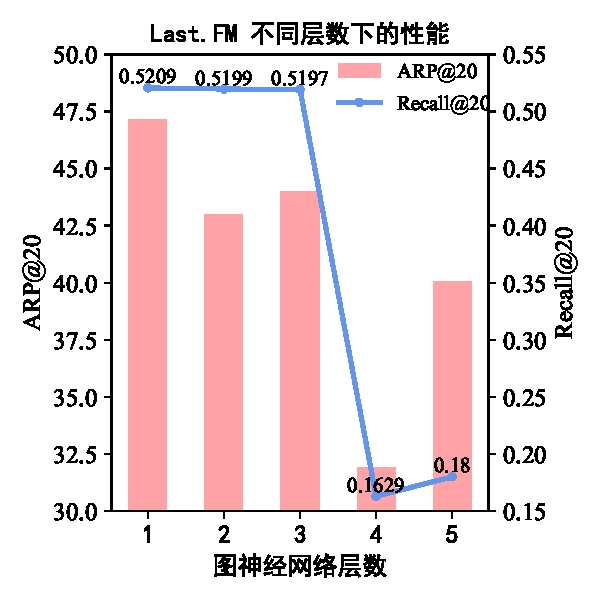
\includegraphics[width=.88\linewidth]{figure/tagcl_param_lastfm_layer.pdf}
%         \caption{layer}
%         \label{fig:tagcl_param_lastfm_layer}
%     \end{subfigure}
%     \begin{subfigure}{0.49\linewidth}
%         \centering
%         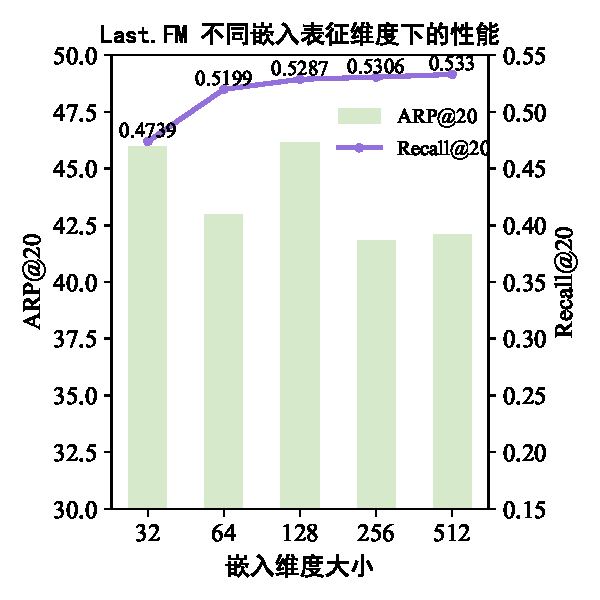
\includegraphics[width=.88\linewidth]{figure/tagcl_param_lastfm_emb.pdf}
%         \caption{emb}
%         \label{fig:tagcl_param_lastfm_emb}
%     \end{subfigure} 
%     \caption{Last.FM 下 TAGCL 的超参数实验}
%     \label{fig:lastfm_tagcl_param}
% \end{figure*}

% \begin{figure*}[!h]
%     \centering
%     \begin{subfigure}{0.49\linewidth}
%         \centering
%         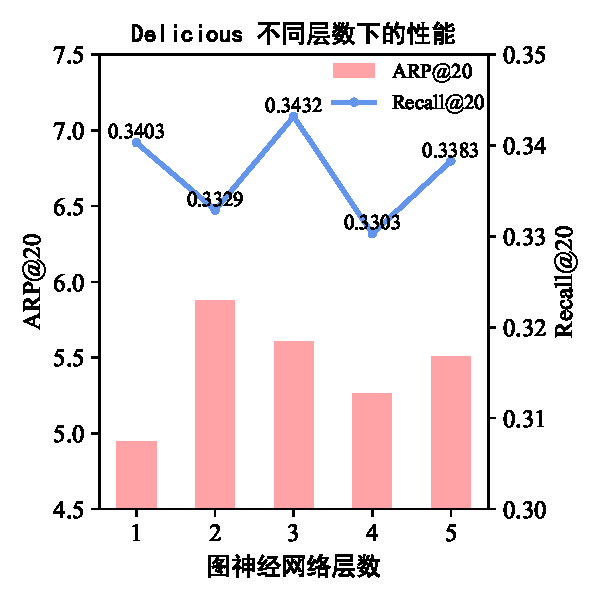
\includegraphics[width=.88\linewidth]{figure/tagcl_param_de_layer.pdf}
%         \caption{layer}
%         \label{fig:tagcl_param_de_layer}
%     \end{subfigure}
%     \begin{subfigure}{0.49\linewidth}
%         \centering
%         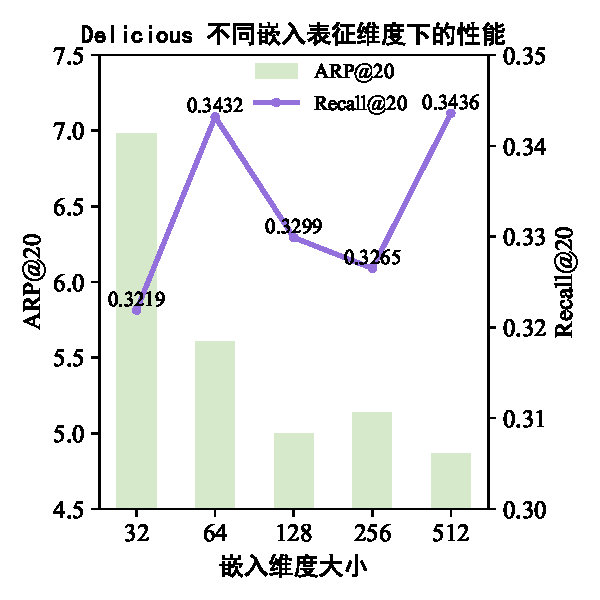
\includegraphics[width=.88\linewidth]{figure/tagcl_param_de_emb.pdf}
%         \caption{emb}
%         \label{fig:tagcl_param_de_emb}
%     \end{subfigure}
%     \caption{Last.FM 下 TAGCL 的超参数实验}
%     \label{fig:de_tagcl_param}
% \end{figure*}

\begin{table}
    \centering
      \caption{模型在 Delicious 上的复杂度}
      \label{tab:complexity}
      \begin{tabular}{c|cc|cc}
      \toprule
      \multirow{2}{*}{\textbf{模型}} &
      \multirow{2}{*}{\makecell[c]{参数量 \\ $(\times 10^6$)}} & 
      \multirow{2}{*}{\makecell[c]{相对 \\ 比率 (\%)}} &
      \multirow{2}{*}{\makecell[c]{推理 \\ 时间 (s)}} & 
      \multirow{2}{*}{\makecell[c]{相对 \\ 比率 (\%)}} \\
       & & & 
       \\
        \midrule
         \begin{tabular}[c]{@{}c@{}}
          LightGCN \\ NGCF  \\ LFGCF \\ GNN-PTR \\ TGCN 
          \end{tabular}
  
          & \begin{tabular}[c]{@{}l@{}}
            \textasciitilde4.33\\  \textasciitilde4.36 \\   \textasciitilde4.55 \\ \textasciitilde4.57 \\ \textasciitilde5.01 
            % 4359168
            % 4334208
            % 5018128
            % 4567104
            % 4558784
          \end{tabular}
          & \begin{tabular}[c]{@{}l@{}}
            -5.18\% \\ -4.58\%   \\ \makecell[c]{-} \\ +0.18\% \\ +9.15\% 
          \end{tabular} 
          & \begin{tabular}[c]{@{}l@{}}
            \textasciitilde0.14 \\ \textasciitilde0.15 \\ \textasciitilde0.13 \\ \textasciitilde0.17 \\ \textasciitilde2.12
          \end{tabular} 
          & \begin{tabular}[c]{@{}l@{}}
            +5.13\% \\ +13.91\% \\ \makecell[c]{-} \\ +16.33\% \\ +93.81\%
          \end{tabular} \\
        \bottomrule
      \end{tabular} 
  \end{table}

  % \begin{table}
  %   \centering
  %   \caption{TAGCL 在 BibSonomy 上的应用}
  %   \label{tab:bibsonomy}
  %   \begin{tabular}{cccccc}
  %     \toprule
  %     \multirow{2}{*}{\textbf{模型}} &
  %     \multicolumn{2}{c}{\textbf{BibSonomy-BM}} &
  %     \multicolumn{2}{c}{\textbf{BibSonomy-BT}} \\
  %     \cline{2-5} 
  %     & \textbf{Rec.@20} & \textbf{ARP.@20} & \textbf{Rec.@20} & \textbf{ARP.@20} \\
  %     \midrule
  %     LightGCN & 0.6117 & 1.53 & 0.4810 & 1.39 \\
  %     TAGCL & 0.6226 & 1.59 & 0.5173 & 1.67 \\
  %     \bottomrule
  %   \end{tabular}
  % \end{table}


  \begin{table}
    \centering
      \caption{模型在 Delicious 上的复杂度}
      \label{tab:complexity}
      \begin{tabular}{c|cc|cc}
      \toprule
      \multirow{2}{*}{\textbf{模型}} &
      \multirow{2}{*}{\makecell[c]{参数量 \\ $(\times 10^6$)}} & 
      \multirow{2}{*}{\makecell[c]{相对 \\ 比率 (\%)}} &
      \multirow{2}{*}{\makecell[c]{推理 \\ 时间 (s)}} & 
      \multirow{2}{*}{\makecell[c]{相对 \\ 比率 (\%)}} \\
       & & & 
       \\
        \midrule
         \begin{tabular}[c]{@{}c@{}}
          LightGCN \\ NGCF  \\ LFGCF \\ GNN-PTR \\ TGCN 
          \end{tabular}
  
          & \begin{tabular}[c]{@{}l@{}}
            \textasciitilde4.33\\  \textasciitilde4.36 \\   \textasciitilde4.55 \\ \textasciitilde4.57 \\ \textasciitilde5.01 
            % 4359168
            % 4334208
            % 5018128
            % 4567104
            % 4558784
          \end{tabular}
          & \begin{tabular}[c]{@{}l@{}}
            -5.18\% \\ -4.58\%   \\ \makecell[c]{-} \\ +0.18\% \\ +9.15\% 
          \end{tabular} 
          & \begin{tabular}[c]{@{}l@{}}
            \textasciitilde0.14 \\ \textasciitilde0.15 \\ \textasciitilde0.13 \\ \textasciitilde0.17 \\ \textasciitilde2.12
          \end{tabular} 
          & \begin{tabular}[c]{@{}l@{}}
            +5.13\% \\ +13.91\% \\ \makecell[c]{-} \\ +16.33\% \\ +93.81\%
          \end{tabular} \\
        \bottomrule
      \end{tabular} 
  \end{table}


  
